\section{A Minimal Model of Nutrient-Mediated Growth Rate Control}
\label{sec:minimal_model}
While the preceding subsections highlight a dominant role for ribosomes in
setting the growth rate, our analysis on the whole has emphasized how the total
proteomic content changes in response to variable growth conditions and
growth rate. In this final section we employ a minimal model of growth rate control
to better understand how this interconnection between ribosomal abundance and
total protein abundance influences the observed growth rate.

Here we propose that cells modulate their protein abundance in direct response
to the availability of nutrients in their environment. As noted earlier,
bacteria can modulate ribosomal activity and its rate of synthesis through the
secondary messenger molecules like (p)ppGpp in poorer nutrient conditions
[Figure \ref{fig:ribosome_limit}(C, inset); \cite{dai2016}] as considered in the work of
\cite{bosdriesz2015}. Importantly, these secondary messengers also cause global
changes in transcriptional and translational activity \citep{hauryliuk2015,
zhu2019, Buke2020}. In \textit{E. coli}, amino acid starvation leads to the
accumulation of de-acylated tRNAs at the ribosome's A-site and a strong increase
in (p)ppGpp synthesis activity by the enzyme RelA \citep{hauryliuk2015}. Along
with this,  there is increasing evidence that (p)ppGpp also acts to inhibit the
initiation of DNA replication and coordinate different cellular processes
\citep{kraemer2019, vadia2017}, providing a potential mechanism for cells to
lower $\langle$\# ori$\rangle$ and maintain a smaller cell size in poorer
nutrient conditions \citep{fernandezcoll2020}.

To consider this quantitatively, we assume that cells modulate their proteome
(total number of peptide bonds $N_\text{pep}$, number of ribosomes $R$, and
ribosomal fraction $\Phi_R$) to better maximize their rate of peptide elongation
$r_t$. The elongation rate $r_t$ will depend on how quickly the ribosomes can
match codons with an amino-acyl tRNA, along with the subsequent steps of peptide
bond formation and translocation. This ultimately depends on the cellular
concentration of amino acids, which we treat as a single effective species,
$[AA]_\text{eff}$. In our model, we determine the the rate of peptide elongation
$r_t$ and achievable growth rate as simply depending on the supply of amino
acids (and, therefore, also amino-acyl tRNAs), through a parameter $r_{AA}$ in
units of AA per second, and the rate of amino acid consumption by protein
synthesis ($r_t \times R \times f_a$). This is shown schematically in
Figure \ref{fig:elongation_rate_model}(A) and derived in the Appendix Section "Derivation
of Minimal Model for Nutrient-Mediated Growth Rate Control". Given our
observation that general protein synthesis and energy production are not limiting, we
assume that other molecular players required by ribosomes such as elongation
factors and GTP are available in sufficient abundance.

In Figure \ref{fig:elongation_rate_model}(B), we illustrate how the elongation rate will
depend on the ribosomal copy number. Here, we have considered an arbitrarily
chosen $r_{AA} = 5\times 10^6$ AA $\cdot$ s$^{-1} \cdot$ \textmu m$^{-3}$ and
$f_a = 1$ for a unit cell volume $V = 1$fL (we provide the interactive figure
Figure \ref{fig:model_explorer} which allows the user to explore
different regimes of this parameter space). At low ribosome copy numbers,
the
observed elongation rate is dependent primarily on $[AA]_\text{eff}$ through
$r_{AA}$ [as $r_t^{\text{max}} \times R \times f_a << r_{AA}$, point (1) in
Figure \ref{fig:elongation_rate_model}(B)]. As the ribosome copy number is increased
such that the amino acid supply rate and consumption rate are nearly equal
[point (2) in Figure \ref{fig:elongation_rate_model}(B)], the observed elongation rate
begins to decrease sharply. When the ribosome copy number is increased even
further, consumption at the maximum elongation rate exceeds the supply rate,
yielding a significantly reduced elongation rate [point (3) in
Figure \ref{fig:elongation_rate_model}{B)]. While the elongation rate will always be
dominated by the amino acid supply rate at sufficiently low ribosome copy
numbers, the elongation rate at larger ribosome abundances can be increased
by tuning $f_a$ such that not all ribosomes are elongating, reducing their
total consumption rate.

\begin{figure}
    \centering{
        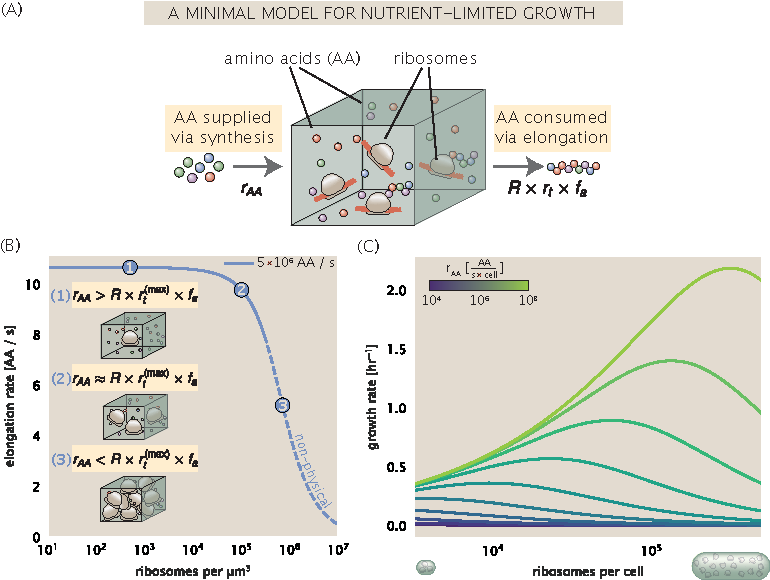
\includegraphics{main_figs/fig12_elongation_model.pdf}
        \caption{\textbf{A minimal model of growth rate control under
        nutrient limitation.} (A) We consider a unit volume of cellular material
        composed of amino acids (colored spheres) provided at a supply rate
        $r_{AA}$. These amino acids are polymerized by a pool of ribosomes
        (brown blobs) at a rate $r_t \times R \times f_a$, where $r_t$ is the
        elongation rate, $R$ is the ribosome copy number in the unit volume, and
        $f_a$ is the fraction of those ribosomes actively translating. (B) The
        observed elongation rate is plotted as a function of the number of ribosomes. The three points correspond to three regimes of
        ribosome copy numbers and are shown schematically on the left-hand side.
        The region of the curve shown as dashed lines represents a non-physical
        copy number, but is shown for illustrative purposes. This curve was
        generated using an amino acid supply rate of $5 \times 10^6$ AA / s,
        a maximal elongation rate of 17.1 AA / s, $f_a = 1$, and a unit cell
        volume of $V = 1$ fL.
        See Appendix Section "Derivation of Minimal Model for Nutrient-Mediated Growth Rate Control" for additional model details. (C) The cellular growth
        rate is plotted as a function of total cellular ribosome copy number for
        different cellular amino acid supply rates, with blue and green curves
        corresponding to low and high supply rates, respectively. As the
        ribosome copy number is increased, so too is the cell size and total
        protein abundance $N_\text{pep}$. We direct the reader to the Supplemental Information
        for discussion on the inference of the relationship between cell
        size, number of peptide bonds, and ribosome copy number.}\label{fig:elongation_rate_model}

    }
\end{figure}

\subsubsection{Optimal Ribosomal Content and Cell Size Depend on Nutrient
Availability and Metabolic Capacity}
To relate elongation rate to growth rate, we constrain the set of parameters
based on our available proteomic measurements; namely, we restrict the values of
$R$, $N_{pep}$, and cell size to those associated with the amalgamated
proteomic data (described in the Appendix Section
"Estimation of Total Protein Content per Cell"). We then consider how changes in the
nutrient conditions, through the parameter $r_{AA}$, influence the maximum
growth rate as determined by Equation \ref{eq:lam_limited}. Figure \ref{fig:elongation_rate_model}(C)
shows how the growth rate depends on the rate of amino acid supply $r_{AA}$ as a
function of the cellular ribosome copy number. A feature immediately apparent is
the presence of a maximal growth rate increases with increasing $r_{AA}$. Importantly, however, there
is an optimum set of $R$, $N_\text{pep}$, and cell size that are strictly dependent on
the value of $r_{AA}$. This shows that increasing the ribosomal concentration
beyond the cell's metabolic capacity will have the adverse consequence of
depleting the supply of amino acids and lead to a concomitant decrease in the elongation
rate $r_t$ [Figure \ref{fig:elongation_rate_model}(B)] and growth rate.
This helps us understand that while it is important for cells to increase
their ribosomal content and cell size in order to increase growth rate,
cells will better maximize their achievable growth rate by tuning these
parameters according to the available nutrient conditions, since this is
ultimately what allows cells to reach the peak for each curve shown in
Figure \ref{fig:elongation_rate_model}(C).

Also of note is the growth rate trends observed at low values of $r_{AA}$
[purple and blue lines in Figure \ref{fig:elongation_rate_model}(C)], representative of
growth in nutrient-poor media. In these
conditions, there no longer exists a peak in growth, at least within the range
of physiologically-relevant ribosome copy numbers considered here. This is a
regime, associated with slower growth rates, where cells limit their pool of
actively translating ribosomes by decreasing $f_a$ (Figure \ref{fig:ribosome_limit}(A),
right-hand panel, inset; \citep{dai2016}), likely due to having excess ribosomes
relative to the cell's metabolic capacity. By reducing the fraction of actively
translating ribosomes, we find that cells instead prioritize maintaining their
pool of available amino acids $[AA]_\text{eff}$ and increasing the achievable
translation elongation rate.
